\begin{figure*}[t]
\centering
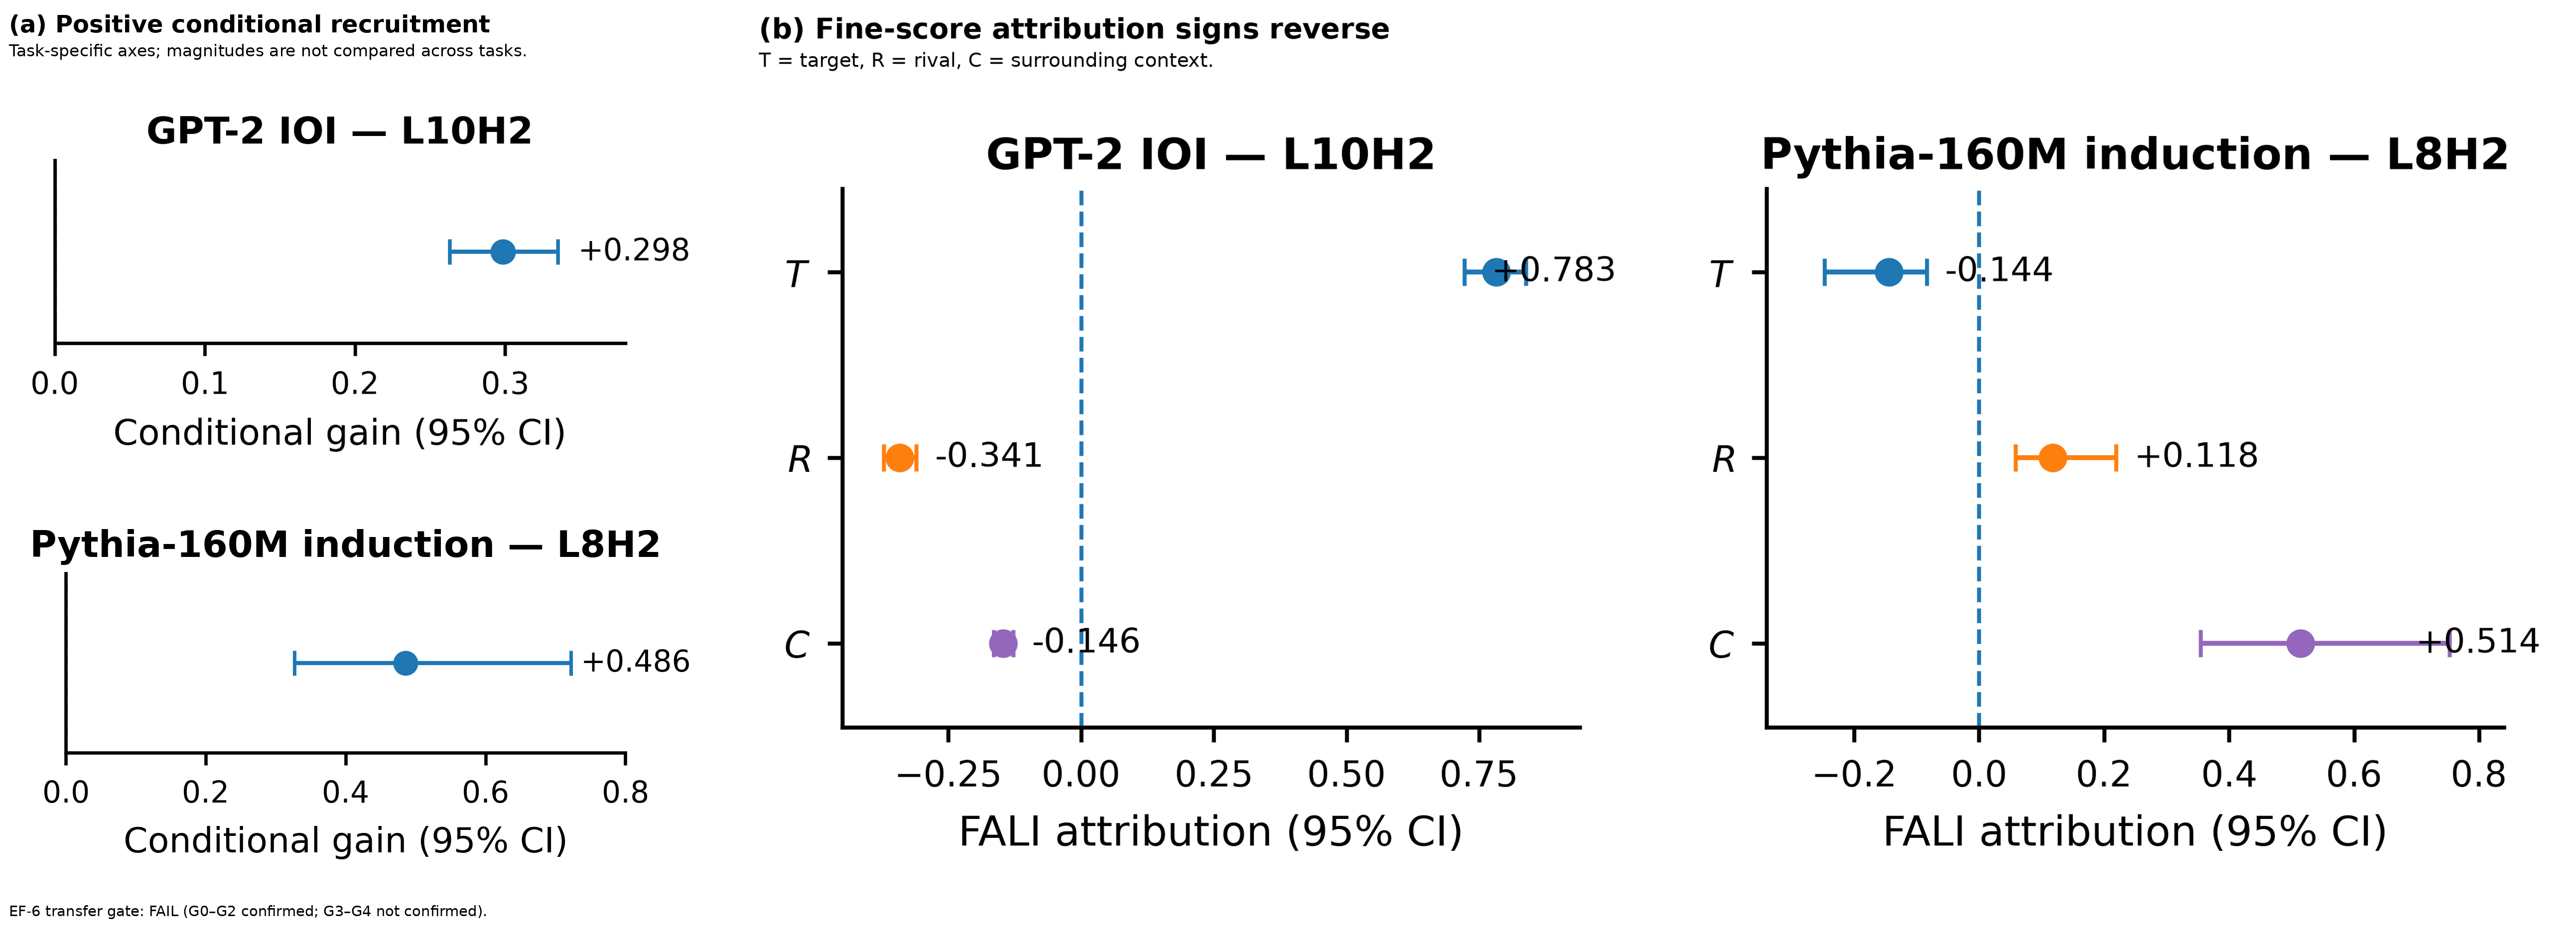
\includegraphics[width=\textwidth]{figures/Fig5.png}
\caption{\textbf{Conditional recruitment occurs in both studied settings, while the preregistered fine-score mechanism does not transfer.}
(a) GPT-2 IOI L10H2 and Pythia-160M induction L8H2 both have positive conditional gain after their respective primary interventions. Separate task-specific axes are used because the underlying utility metrics differ; numerical magnitudes should not be compared across tasks.
(b) The observed fine attribution signs reverse: GPT-2 is target-positive/rival-negative, whereas Pythia is target-negative/rival-positive; their surrounding-context contributions also differ in sign. Points are exact balanced means and intervals are the preregistered 95\% bootstrap confidence intervals for each experiment. The Pythia transfer test confirms induction behavior, primary-head importance, and positive conditional recruitment (G0--G2), while G3--G4 are not confirmed, yielding overall EF-6 FAIL. This is a failed mechanism-transfer hypothesis, not a failed recruitment result.}
\label{fig:cross-setting-reversal}
\end{figure*}
